\section{Fluxionnal compiler} \label{section:compiler}

Web applications are currently, mostly written in Java.
The langage proposes both data encapsulation in objects and a threading model that allows the development of parallel applications.
But, this approach is error-prone, and leads to deadlocks and other synchronization problems \cite{Adya2002}.
Since 2009, \textit{Node.js} proposes an alternative to this model.
It provides a Javascript execution environment for real-time web applications, with data encapsulation in modules, and a concurrency model based on an event-loop.
We focus on this promising environment for its initial simplicity and efficiency.
We develop a compiler that transforms a \textit{Node.js} application into a fluxional system compliant with the architecture described in section \ref{section:model}.
Our compiler uses a new approach to find independent parts in \textit{Node.js} applications.
It finds rupture points that represent boundaries between fluxions.
We do not target all Javascript Web-based application as this work is only a proof of concept for the compilation.
Our goal is to compile a few real applications without modifying their code, so as to validate this approach.

Section \ref{section:compiler:analyzer} define rupture points, and explains how the compiler detects them.
Section \ref{section:compiler:linker} explains how the compiler distribute the central memory into isolated fluxions.

\subsection{Analyzer} \label{section:compiler:analyzer}

\subsubsection{Rupture points} \label{section:compiler:analyzer:rupture}

A rupture point is a call of a loosely coupled function.
It is an asynchronous call without subsequent synchronization with the caller.
In \textit{Node.js}, I/O operations are asynchronous functions.
That is a function call that resumes immediately, with a function to process later the result of the operation : the callback.
The callback is loosely coupled with the initial caller, because they are not executed on the same call stack.
This rupture in the call stacks marks out the separation between two independent application parts.
In the \textit{Node.js} environment, these two application parts are executed sequentially on the same thread to avoid concurrent memory accesses.
But the compiler intends to isolate their memories to reveal a pipeline parallelism, as defined in\cite{Gordon2006}.

A callback is a function passed as a parameter to a function call.
It is invoked by the callee to continue the execution with data not available in the caller context.
We distinguish three kinds of callbacks.

\textbf{Iterators} are functions called for each item in a set, often synchronously.

\textbf{Listeners} are functions called asynchronously for each event in a stream.

\textbf{Continuations} are functions called asynchronously once a result is available.

There is two types of asynchronous callbacks : listeners and continuations.
Similarly, there is two types of rupture point, respectively \textit{start} and \textit{post}.

\textbf{Start rupture points} are indicated by listeners. They are on the border between the application and the outside, continuously receiving incoming user requests.
An example of a start rupture point is in listing \ref{lst:source}, between the call to \texttt{app.get()}, and its listener \texttt{handler}.
These rupture points indicate the input of a data stream in the program, and the beginning of a chain of fluxions to process this stream.

\textbf{Post rupture points} are indicated by continuations.
They represent a continuity in the execution flow after an asynchronous operation yielding a unique result, such as reading a file, or querying a database.
An example of a post rupture points is in listing \ref{lst:source}, between the call to \texttt{fs.readFile()}, and its continuation \texttt{reply}.

% The compilation results for these rupture points is illustrated in listing \ref{lst:ex-jsres} and explained in section \ref{section:example}.

The isolation of the execution between the asynchronous call and the callback is illustrated figure \ref{fig:basicrp}. The interface line represent the limit between two fluxions. It means that the upstream fluxion sends a message to the downstream fluxion to continue the execution with the callback.

\begin{figure}[h!]
\begin{center}
  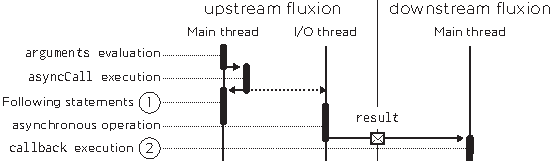
\includegraphics[width=\linewidth]{ressources/basicrp.pdf}
  \caption{The rupture point interface is placed between the asynchronous operation and the callback in between the two call stacks.}
  \label{fig:basicrp}
\end{center}
\end{figure}

\subsubsection{Detection}

Listeners and continuations are asynchronous because they are called asynchronously, and not because they are defined differently than any other function.
Therefore, the identification of a rupture point holds on the callee, not on the callback.
In listing \ref{lst:source}, the two rupture points are identified because of \texttt{app.get} and \texttt{fs.readFile}, not because of \texttt{handler} and \texttt{reply}.
The asynchronism is provided by the execution engine, not the language.
Therefore, it is impossible to identify an asynchronous function from a synchronous function based on their syntax.
The compiler uses a list of common asynchronous callee, like the \texttt{express} and file system methods.
This list can be augmented to match asynchronous callee individually for any application.

% The compiler is prebuilt knowing some module names exposing asynchronous functions, like the \textit{express} and the \textit{fs} module in listing \ref{lst:rupturepoints}.
% To detect asynchronous calls, the compiler keeps a list of variables holding these modules.
% In listing \ref{lst:rupturepoints}, the compiler adds both variables \texttt{app} and \texttt{fs} in this list.
% When the compiler encounters a call expression, it compares its callee name with this list to spot asynchronous functions.

After the identification of the callee, the callback needs to be identified as well to be encapsulated in the downstream fluxion.
For each asynchronous call detected, the compiler test if one of the arguments is of type \texttt{function}.
Some callback functions are declared \textit{in situ}, and are trivially detected.
For variable identifier, and other expressions, the compiler tries to detect their type by tracking their assignations and modification.
Missing callbacks by false negatives in the detection is sub-optimal, but false positives are more critical, as they eventually introduce bugs.
Therefore, the detection needs to be as accurate as possible to screen out false positives.
It walks an intermediate representation of the source code to spot the statements modifying a variable.
From this intermediate representation, the variable tracker builds a dependency graph which helps the analyzer to detect the type of a variable at a certain point in the execution.
The variable tracker is still in early development and is limited to only a few cases.
In future works, our tracking method would be inspired from the points-to analysis \cite{Wei2014}.

\subsection{Linker} \label{section:compiler:linker}

In a stream processing, there is roughly two kinds of usage of the global memory : data and state \cite{Fernandez2014a}.
Naively, the data represent a communication channel between different point in the application space, and the state represents a communication channel between different instant in time.
The data flow from stage to stage through the pipeline, and are never stored on any fluxion. In the source application, it is stored in the heap, only as a buffer between the different callbacks.
The state, on the other hand, remains in the memory to impact the future behaviors of the application.
State might be shared by several parts of the application.
So, the identification of rupture points is not enough for a fluxion to be isolated, and its execution parallelized.
The compiler also needs to analyze the memory accesses to identify which part of the state is needed by each fluxion, and allow their coordination.

\subsubsection{Scope isolation}

In Javascript, the memory is organized in scopes.
They are nested one in the other up to the all-enclosing global scope.
Each function creates a new scope containing variables local to itself.
It is chained to the scope of the parent function, so that the child function can access variables in the scope of the parent functions, up to the global scope.
However, the scope of the function inside a fluxion is isolated from its ancestors.

A rupture point eventually breaks a chain of scopes.
When it is between a child scope and its parent, it makes the child unable to access its parent as expected.
The parent is in the upstream fluxion, and the child in the downstream fluxion.
%For example, callback functions declared \textit{in situ}.
Or when it is between a closure, and its definition context.
The definition context is in the upstream fluxion and the closure in the downstream fluxion.
If this situations aren't resolved, they introduce errors in the compilation result.
The linker analyzes how scopes are distributed among the fluxions to identify how the variables broken onto several fluxions are used in the upstreams and downstreams fluxions.
At the end of this analysis, the compiler knows for every variable, if it is read or modified inside each fluxion.

However, scopes are an abstract representation of the memory, it is only the surface.
Internally, the heap is a global memory without any fencing.
A variable in one scope can point to the same object as another variable in another scope.
If the first variable is modified, the modification propagates to the second variable, without this second variable being visibly modified.
This situation produces side-effects between the two scopes.
We call these side-effects scope leaking.
If these two scopes are isolated on two different workers, the side-effects are unable to propagate as expected.
We identified three basic situations leading to scope leaks.

\paragraph{Assignment}

If a variable is assigned the object of another variable, there is possibly side effects between these two variables.
It is illustrated in listing \ref{lst:assignment}.
The variable \texttt{a} is never modified visibly, yet, it is modified through the variable \texttt{b}.

\begin{code}[js, caption={Example of a scope leak due to assignment},label={lst:assignment}]
var a = {item: 'unchanged'};
var b = a;

async_fn(function callback() {
  b.item = 'changed';
  console.log(a.item); // 'changed';
})
\end{code}

\paragraph{Function call}

When a variable containing an object is passed as an argument to a function call, it is assigned to a different variable as a parameter inside the function scope.
There is possibly side effects between these two variables.
It is illustrated in listing \ref{lst:argument}.
The variable \texttt{a} is passed as an argument to the function \texttt{async\_fn}.
The function \texttt{callback} is then called by \texttt{async\_fn} with the object from \texttt{a} as an argument.
The variable \texttt{a} is never modified visibly, yet it is modified through the variable \texttt{b}.

\begin{code}[js, caption={Example of a scope leak due to a function call},label={lst:argument}]
var a = {item: 'unchanged'};

async_fn(function callback(b) {
  b.item = 'changed';
  console.log(a.item); // 'changed';
}, a);
\end{code}

\paragraph{Closure}

A closure is a function which conserves its access over its creation context.
When the closure is called, it can modify this creation context from outside the scope of this creation context.
There is possibly side effects from outside this scope.
It is illustrated in listing \ref{lst:closure}.
The variable \texttt{a} is only modified visibly inside an anonymous function.
This anonymous function is returned to be assigned in the variable \texttt{closure}.
The variable \texttt{a} is modified when \texttt{closure} is called.

\begin{code}[js, caption={Example of a scope leak due to a closure},label={lst:closure}]
function closureFactory() {
  var a = {item: 'unchanged'};
  return function() {
    a.item = 'changed';
  }
}

var closure = closureFactory();

async_fn(function() {
  closure();
  // inside closureFactory : a.item === 'changed';
});
\end{code}

Our compiler is currently in early stage of development.
The scope analysis previously presented is unable to take these scope leaking into account.
It is unable to analyze the memory deeply enough to provide a sound and complete analysis.
Therefore it might lead to runtime errors.
Moreover, we present only basic situations of scope leaking.
Javascript exposes many other features leading to scope leaking, like prototype inheritance.

\subsubsection{State sharing}

Depending on the result of the previous analysis on the variable usage through scopes, there is three different ways the compiler can resolve the conflict.


\paragraph{Scope}
If a variable is modified inside only one fluxion, then it can be part of the context of this fluxion.
The fluxion has an exclusive access to it.
If the context of a fluxion doesn't contains references shared with other fluxions, then it can be isolated on its own worker for its execution to be parallelized.

\paragraph{Stream}
If a variable is modified inside one fluxion, but read inside at least one downstream fluxion, then it can be part of the message to be sent to the downstream fluxions.

It is possible to stream variables only to downstream flux\-ions.
Indeed, if the fluxion retro propagates the variable for an upstream fluxion to read, the upstream fluxion might use the old version while the new version is on its way.
To avoid such race conditions, we avoid retro propagation.

Additionally, it is currently impossible to stream variables containing closures.
Indeed, it is impossible to serialize closure from within Javascript.
As the fluxionnal execution model is currently confined inside the Javascript execution environment, it is unable to send closures from one worker to the other.

\paragraph{Share}
If a variable is needed for modification by more than one fluxion, or is read by an upstream fluxion, then it needs to be synchronized between the fluxions.
The synchronization of a distributed memory is a well-known subject, with Brewer's conjecture \cite{Gilbert2002}, and the BASE semantics\cite{Fox1997}.
However, we currently choose to not allow such synchronization between workers.
All the fluxions sharing a variable are gathered on the same worker to disallow parallel access on their shared memory.
Similarly, if a fluxion shares references or closures with other fluxions, either in its context, or streams, they need to be hosted on the same worker.


















\endinput

























\subsection{Compilation example} \label{section:example}

% For copyright reason, the compiler source code is kept private along with the tests we used.
To illustrate the compiler features, we compiled the application used as an example for the execution model in section \ref{section:model}.
The source and compiled results of this application are available on github\cite{flx-example}.
The compiler source code is the property of Worldline, and is not publicly available, but we are planning of releasing it as an open source project in the future.

To test the source or the result of the compilation, one would launch respectively \texttt{source.js} or \texttt{result.js} with \texttt{node} and check the service available at \texttt{localhost:8080}.
Both executable needs their dependencies to be resolved with \texttt{npm} before execution.
\begin{verbatim}
git clone https://github.com/etnbrd/flx-example
cd flx-example
npm install
node result.js
open http://localhost:8080
\end{verbatim}

The file \texttt{source.js}, in listing \ref{lst:ex-source}, is the source of this compilation example.
This application sends back its own source along with a download counter.
The processing chain of function is : $\texttt{get} \to \texttt{handler} \to \texttt{readFile} \to \texttt{reply} \to \texttt{send}$.
It uses two asynchronous function call with \textit{in situ} callback, one to listen for user requests and one to read its own source, respectively \texttt{app.get} line 5 and \texttt{fs.read} line 6.
It uses a global variable to increment the download counter defined line 3.
This global variable is used only in the \texttt{reply} function, line 7 and 9.

\includecode{js,
  caption={Source of the compilation example},
  label={lst:ex-source}
}
{../../flx-example/source.js}

The result of the compilation into our high-level language is in the file \texttt{result.flx}, presented in listing \ref{lst:ex-flxres}.
The analyzer detects both asynchronous calls as rupture points.
The first one is a \textit{start} rupture point, associated with the \texttt{app.get} asynchronous function call which makes the callback \texttt{handler} listen for the stream of user requests. 
The second one is a \textit{post} rupture point, associated with the \texttt{fs.readFile} asynchronous function call which reads the source file and hands it to the callback \texttt{reply}.
These two rupture points result in three application parts.
The first application part is encapsulated in the root fluxion, named after the filename, \texttt{source.js}, line 1.
It initializes the system to route the user requests to the fluxion \texttt{handler-1000}, line 8.
This second fluxion reads the file, and sends the result to the next and last fluxion \texttt{reply-1001}, line 14.
We can identify the processing chain of functions in this chain of fluxion.

\begin{center}
\texttt{source.js} (\texttt{get})\\
$\downarrow$\\
\texttt{handler-1000} (\texttt{handler}, \texttt{readFile})\\
$\downarrow$\\
\texttt{reply-1001} (\texttt{reply}, \texttt{send})
\end{center}

The linker detects that the fluxion \texttt{reply-1001} needs two variable to send the result back to the user, \texttt{res} and \texttt{count}.
The variable \texttt{res} depends on the user connection and is initialized for each new request.
It needs to be part of the \textit{signature} of the message transfered to the last fluxion.
The variable \texttt{count} is global, and the \texttt{reply} function in the fluxion \texttt{reply-1001} needs to increment it at each new request.
This global variable is in the \textit{scope} of only this application part, so the compiler stores it in the \textit{context} of this fluxion.
The division by the compiler of this application is illustrated figure \ref{fig:flux-3}.
This result is very similar to the manual division illustrated figure \ref{fig:fluxions}, as expected.

\includecode{flx,
  caption={High level fluxional language result of the compilation example},
  label={lst:ex-flxres}
}
{../../flx-example/result.flx}

\begin{figure}[h!]
\begin{center}
  \includegraphics[width=\linewidth]{ressources/flux-3.pdf}
  \caption{Division of the listing \ref{lst:ex-flxres} into three application parts. This result is similar to the manual division illustrated in figure \ref{fig:fluxions}}
  \label{fig:flux-3}
\end{center}
\end{figure}

The compiler also produces an executable targeting a simple implementation of the fluxional execution model.
This result is in the file \texttt{result.js}, presented in listing \ref{lst:ex-jsres}.
The \textit{root} fluxion is not registered because it doesn't need to receive any message by another fluxion, it only initializes the application.
The two following fluxions are registered in the messaging system.
This registration encapsulates the processing function in a \texttt{capsule} function.
The \textit{special rupture points} implies the asynchronous call to be in the downstream fluxion.
The \texttt{capsule} function encapsulates the asynchronous call from a \textit{special rupture points} or the callback from \textit{basic rupture points} in a unified processing function.

The original callback is replaced with a \texttt{placeholder} function, line 3, sending the \textit{start} message to \texttt{handler-1000}.
Line 17, \texttt{handler-1000} pushes the user request \texttt{res} in the message and \texttt{post} it directly to \texttt{reply-1001}.
Because there is a special rupture point between \texttt{handler-1000} and \texttt{reply-1001}, the asynchronous call is moved to \texttt{reply-1001} and the \texttt{post} function doesn't replace the callback, like the placeholder line 3, but is directly called.
Finally, \texttt{reply-1001} receives the message containing the user request and reads the file.
The callback of this asynchronous operation, \textit{reply} function, line 27, increments the variable \texttt{counter}, line 28, and sends the reply, line 30.

\includecode{flx,
  caption={Result of the compilation example targeting the fluxional execution model},
  label={lst:ex-jsres}
}
{../../flx-example/result.js}

\subsection{Limitations}

This compiler aims at transforming a subset of Javascript web applications presenting a specific syntax and design.
In this section, we describe briefly the current limitations of our compiler and how we plan to overcome them in future works.

\begin{itemize}
  \item Variables poorly encapsulated or used too broadly tighten dependencies accross the code, and might result in a coarser division of the application.
  \item The compilation silently fails if a variable holding a callback or a module is overwritten, or not defined in the declaration.
        The variable tracker is unable to track accurately all the modification of a variable to detect these situations which may lead the compiler either to miss rupture points, or to detect non existing one.
  \item The compiler is unable to track a dynamically resolved value, even if the value is deducible statically.
        If this variable is used in a potential rupture point, the compiler screens it out.
  \item The Javascript language offers rich composition possibilities leading to many corner cases.
        The compiler is not robust enough to understand all corner cases.
        For example, the \textit{express} module is only detected if initialized like in listing \ref{lst:rupturepoints}.
\end{itemize}
There may be other limitations we aren't aware of.

The three last limitations described above are caused by the variable tracker - described in section \ref{section:analyzer} - being in an early stage of development.
We are currently in the process of improving the robustness of the compiler to extend the subset of compilable applications.

% We believe that our work will keep scalability concerns out of the way for the development team, who could then focus on the core logic of their application.
% In future developments of this project, we aim at making application dynamically reactive to the load of user requests.
% By monitoring only the input stream, the \texttt{start} rupture points, we believe it is possible to infer the load propagation through the application.
% Using analogy with fluid dynamics, each fluxion is like a pipe, traversed by a fluid of user requests.
% The input and output throughput of this pipe could be calibrated before production use, generating an approximative model of the application reaction to input load.
% Using this model, we want to make the application's reorganize itself in a cluster to handle pikes in the user request throughput.
